% Mapa conceptual de lecturas — IPre Sueño-Vigilia y Aprendizaje Composicional
% Compilar:  pdflatex mapa_papers.tex  &&  pdftocairo -svg mapa_papers.pdf mapa_papers.svg
\documentclass[tikz,border=8pt]{standalone}
\usepackage[utf8]{inputenc}
\usepackage[T1]{fontenc}
\usepackage{helvet}
\renewcommand{\familydefault}{\sfdefault}
\usetikzlibrary{arrows.meta,positioning,calc,backgrounds}

% ---------- Paleta por línea temática ----------
\definecolor{cProg}{HTML}{C0392B}   % síntesis de programas
\definecolor{cMDL}{HTML}{8E6C00}    % simplicidad / MDL
\definecolor{cVI}{HTML}{1F5FA8}     % inferencia variacional
\definecolor{cDisc}{HTML}{6B3FA0}   % latentes discretos
\definecolor{cColl}{HTML}{0E7C6B}   % colapso posterior
\definecolor{cRL}{HTML}{B85C00}     % RL / world models
\definecolor{cEdge}{HTML}{3C3C3C}
\definecolor{cGray}{HTML}{808080}

% ---------- Geometría ----------
\newcommand{\dx}{3.9}    % separación horizontal entre columnas (cm)
\newcommand{\dy}{3.0}    % separación vertical entre carriles (cm)

\tikzset{
  paper/.style={
    draw=#1, very thick, fill=#1!12, rounded corners=3pt,
    text width=2.9cm, align=center, inner sep=4pt,
    font=\scriptsize, minimum height=1.45cm},
  aux/.style={  % citado en el apunte, no adjuntado
    draw=#1, thick, dashed, fill=white, rounded corners=3pt,
    text width=2.9cm, align=center, inner sep=4pt,
    font=\scriptsize, minimum height=1.45cm},
  rel/.style={-{Stealth[length=2.4mm]}, cEdge, thick, rounded corners=6pt},
  con/.style={-{Stealth[length=2.4mm]}, cEdge, thick, dashed, rounded corners=6pt},
  lbl/.style={font=\tiny\itshape, fill=white, fill opacity=0.92, text opacity=1,
              inner sep=1.3pt, text=black!85, align=center},
}
% \tit{título}{autores}{año}
\newcommand{\tit}[3]{\textbf{#1}\\[1pt]{\color{black!65}#2}\\[1pt]\textbf{#3}}

\begin{document}
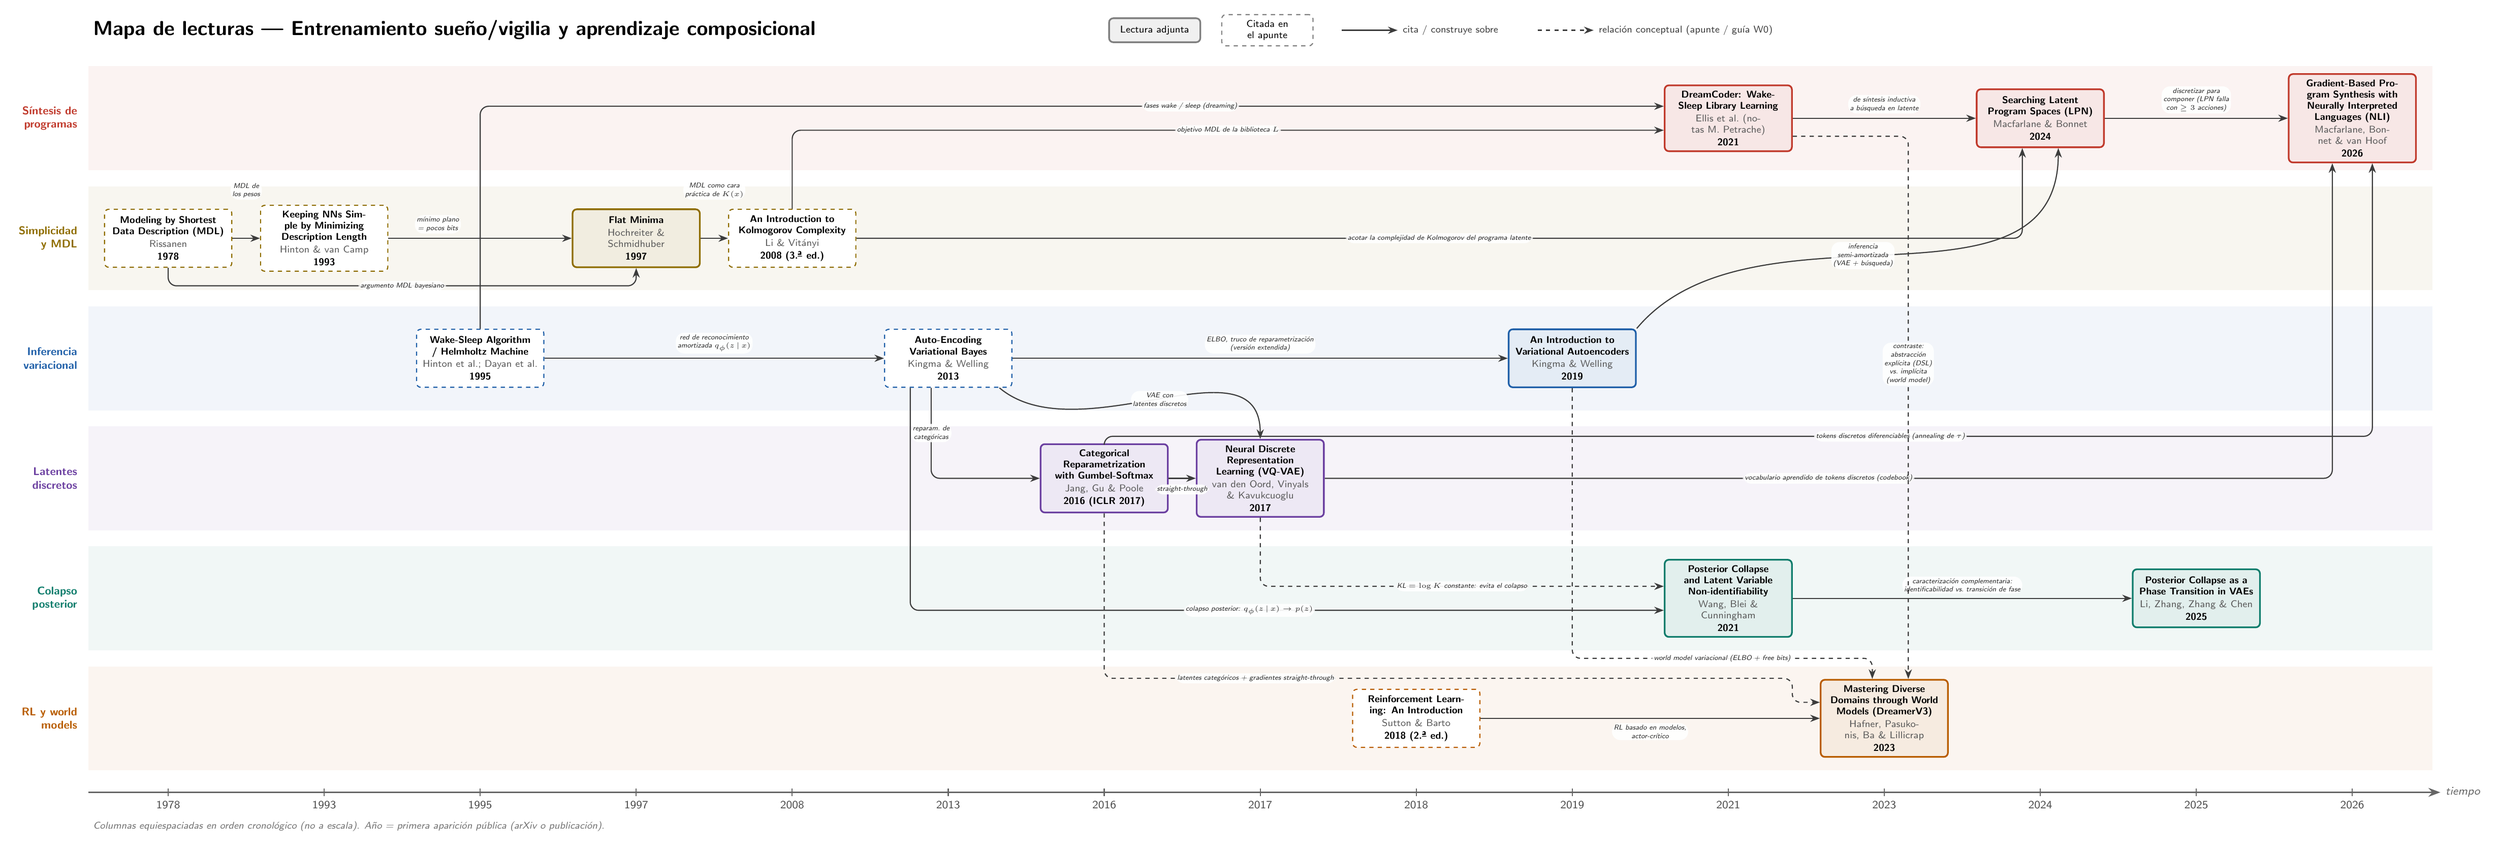
\begin{tikzpicture}

% ---------- Carriles (y) ----------
\pgfmathsetmacro{\yP}{0}
\pgfmathsetmacro{\yM}{-\dy}
\pgfmathsetmacro{\yV}{-2*\dy}
\pgfmathsetmacro{\yD}{-3*\dy}
\pgfmathsetmacro{\yC}{-4*\dy}
\pgfmathsetmacro{\yR}{-5*\dy}

% ================= NODOS (columna = orden cronológico) =================
\node[aux=cMDL]   (mdl)   at (0*\dx,\yM) {\tit{Modeling by Shortest Data Description (MDL)}{Rissanen}{1978}};
\node[aux=cMDL]   (hvc)   at (1*\dx,\yM) {\tit{Keeping NNs Simple by Minimizing Description Length}{Hinton \& van Camp}{1993}};
\node[aux=cVI]    (helm)  at (2*\dx,\yV) {\tit{Wake-Sleep Algorithm / Helmholtz Machine}{Hinton et al.; Dayan et al.}{1995}};
\node[paper=cMDL] (flat)  at (3*\dx,\yM) {\tit{Flat Minima}{Hochreiter \& Schmidhuber}{1997}};
\node[aux=cMDL]   (kolm)  at (4*\dx,\yM) {\tit{An Introduction to Kolmogorov Complexity}{Li \& Vit\'anyi}{2008 (3.\textordfeminine\ ed.)}};
\node[aux=cVI]    (aevb)  at (5*\dx,\yV) {\tit{Auto-Encoding Variational Bayes}{Kingma \& Welling}{2013}};
\node[paper=cDisc](gumb)  at (6*\dx,\yD) {\tit{Categorical Reparametrization with Gumbel-Softmax}{Jang, Gu \& Poole}{2016 (ICLR 2017)}};
\node[paper=cDisc](vqvae) at (7*\dx,\yD) {\tit{Neural Discrete Representation Learning (VQ-VAE)}{van den Oord, Vinyals \& Kavukcuoglu}{2017}};
\node[aux=cRL]    (sb)    at (8*\dx,\yR) {\tit{Reinforcement Learning: An Introduction}{Sutton \& Barto}{2018 (2.\textordfeminine\ ed.)}};
\node[paper=cVI]  (vaei)  at (9*\dx,\yV) {\tit{An Introduction to Variational Autoencoders}{Kingma \& Welling}{2019}};
\node[paper=cProg](dc)    at (10*\dx,\yP) {\tit{DreamCoder: Wake-Sleep Library Learning}{Ellis et al.\ (notas M.\ Petrache)}{2021}};
\node[paper=cColl](wang)  at (10*\dx,\yC) {\tit{Posterior Collapse and Latent Variable Non-identifiability}{Wang, Blei \& Cunningham}{2021}};
\node[paper=cRL]  (dv3)   at (11*\dx,\yR) {\tit{Mastering Diverse Domains through World Models (DreamerV3)}{Hafner, Pasukonis, Ba \& Lillicrap}{2023}};
\node[paper=cProg](lpn)   at (12*\dx,\yP) {\tit{Searching Latent Program Spaces (LPN)}{Macfarlane \& Bonnet}{2024}};
\node[paper=cColl](phase) at (13*\dx,\yC) {\tit{Posterior Collapse as a Phase Transition in VAEs}{Li, Zhang, Zhang \& Chen}{2025}};
\node[paper=cProg](nli)   at (14*\dx,\yP) {\tit{Gradient-Based Program Synthesis with Neurally Interpreted Languages (NLI)}{Macfarlane, Bonnet \& van Hoof}{2026}};

% ================= ARCOS =================
% Coordenadas auxiliares de "pasillos"
\pgfmathsetmacro{\topP}{\yP+1.0}      % pasillo superior del carril de programas
\pgfmathsetmacro{\topD}{\yD+1.05}     % pasillo superior del carril discreto
\pgfmathsetmacro{\topR}{\yR+1.05}     % pasillo superior del carril RL

% --- Simplicidad / MDL ------------------------------------------------
\draw[rel] (mdl) -- node[lbl,above=0.95cm] {MDL de\\los pesos} (hvc);
\draw[rel] (hvc) -- node[lbl,above=3pt,pos=0.27] {mínimo plano\\= pocos bits} (flat);
\draw[rel] (mdl.south) -- ++(0,-0.45) -| node[lbl,pos=0.25] {argumento MDL bayesiano} (flat.south);
\draw[rel] (flat) -- node[lbl,above=0.95cm] {MDL como cara\\práctica de $K(x)$} (kolm);

% Kolmogorov/MDL -> DreamCoder y LPN
\draw[rel] (kolm.north) |- node[lbl,pos=0.75] {objetivo MDL de la biblioteca $L$} ($(dc.west)+(0,-0.3)$);
\draw[rel] (kolm.east) -- (12*\dx-0.45,\yM)
     node[lbl,pos=0.5] {acotar la complejidad de Kolmogorov del programa latente}
     -- ($(lpn.south)+(-0.45,0)$);

% --- Inferencia variacional --------------------------------------------
\draw[rel] (helm) -- node[lbl,above=3pt] {red de reconocimiento\\amortizada $q_\phi(z\,|\,x)$} (aevb);
\draw[rel] (helm.north) |- node[lbl,pos=0.8] {fases wake / sleep (dreaming)} ($(dc.west)+(0,0.3)$);
\draw[rel] (aevb) -- node[lbl,above=3pt] {ELBO, truco de reparametrización\\(versión extendida)} (vaei);

\draw[rel] (aevb.-120) |- node[lbl,pos=0.25] {reparam.\ de\\categóricas} (gumb.west);
\draw[rel] (aevb.-30) to[out=-40,in=90] node[lbl,pos=0.5] {VAE con\\latentes discretos} (vqvae.north);

% AEVB -> Wang (pasillo inferior del carril de colapso)
\draw[rel] ($(aevb.south)+(-0.95,0)$) -- (5*\dx-0.95,\yC-0.3)
      -- node[lbl,pos=0.45] {colapso posterior: $q_\phi(z\,|\,x)\to p(z)$} ($(wang.west)+(0,-0.3)$);
\draw[con] (vqvae.south) -- (7*\dx,\yC+0.3)
      -- node[lbl,pos=0.5] {KL $=\log K$ constante: evita el colapso} ($(wang.west)+(0,0.3)$);

\draw[rel] (vaei.north east) to[out=50,in=-90] node[lbl,pos=0.45] {inferencia\\semi-amortizada\\(VAE + búsqueda)} ($(lpn.south)+(0.45,0)$);
\draw[con] (vaei.south) -- (9*\dx,\yR+1.5) -- node[lbl,pos=0.5] {world model variacional (ELBO + free bits)} (11*\dx-0.3,\yR+1.5) -- ($(dv3.north)+(-0.3,0)$);

% --- Latentes discretos -------------------------------------------------
\draw[rel] (gumb) -- node[lbl,below=4pt] {straight-through} (vqvae);
\draw[con] (gumb.south) -- (6*\dx,\yR+1.0) -- (11*\dx-2.3,\yR+1.0)
      node[lbl,pos=0.22] {latentes categóricos + gradientes straight-through}
      -- (11*\dx-2.3,\yR+0.4) -- ($(dv3.west)+(0,0.4)$);
\draw[rel] (vqvae.east) -- (14*\dx-0.5,\yD)
      node[lbl,pos=0.5] {vocabulario aprendido de tokens discretos (codebook)}
      -- ($(nli.south)+(-0.5,0)$);
\draw[rel] (gumb.north) -- (6*\dx,\topD) -- (14*\dx+0.5,\topD)
      node[lbl,pos=0.62] {tokens discretos diferenciables (annealing de $\tau$)}
      -- ($(nli.south)+(0.5,0)$);

% --- Colapso posterior --------------------------------------------------
\draw[rel] (wang) -- node[lbl,above=3pt] {caracterización complementaria:\\identificabilidad vs.\ transición de fase} (phase);

% --- RL -----------------------------------------------------------------
\draw[rel] (sb.east) -- node[lbl,below=3pt] {RL basado en modelos,\\actor-crítico} (dv3.west);

% --- Síntesis de programas ----------------------------------------------
\draw[rel] (dc) -- node[lbl,above=3pt] {de síntesis inductiva\\a búsqueda en latente} (lpn);
\draw[rel] (lpn) -- node[lbl,above=3pt] {discretizar para\\componer (LPN falla\\con $\ge 3$ acciones)} (nli);
\draw[con] ($(dc.east)+(0,-0.45)$) -- (11*\dx+0.6,\yP-0.45)
      -- node[lbl,pos=0.42] {contraste:\\abstracción\\explícita (DSL)\\vs.\ implícita\\(world model)}
      ($(dv3.north)+(0.6,0)$);

% ================= CARRILES Y EJE TEMPORAL =================
\begin{scope}[on background layer]
  \foreach \y/\c/\t in {\yP/cProg/{Síntesis de\\programas},
                        \yM/cMDL/{Simplicidad\\y MDL},
                        \yV/cVI/{Inferencia\\variacional},
                        \yD/cDisc/{Latentes\\discretos},
                        \yC/cColl/{Colapso\\posterior},
                        \yR/cRL/{RL y world\\models}} {
    \fill[\c!6] (-2.0,\y-1.3) rectangle (14*\dx+2.0,\y+1.3);
    \node[font=\footnotesize\bfseries, text=\c, align=right, anchor=east]
         at (-2.15,\y) {\t};
  }
\end{scope}

% eje de tiempo
\pgfmathsetmacro{\yA}{\yR-1.85}
\draw[-{Stealth[length=3mm]}, thick, black!60] (-2.0,\yA) -- (14*\dx+2.2,\yA)
  node[right, font=\footnotesize\itshape, black!60] {tiempo};
\foreach \i/\yr in {0/1978,1/1993,2/1995,3/1997,4/2008,5/2013,6/2016,7/2017,
                    8/2018,9/2019,10/2021,11/2023,12/2024,13/2025,14/2026} {
  \draw[black!60, thick] (\i*\dx,\yA+0.1) -- (\i*\dx,\yA-0.1);
  \node[below, font=\footnotesize, black!70] at (\i*\dx,\yA-0.1) {\yr};
}
\node[font=\scriptsize\itshape, black!55, anchor=north west] at (-2.0,\yA-0.6)
  {Columnas equiespaciadas en orden cronológico (no a escala). Año = primera aparición pública (arXiv o publicación).};

% ================= TÍTULO Y LEYENDA =================
\begin{scope}[shift={(-2.0,\yP+2.2)}]
  \node[font=\Large\bfseries, anchor=west] at (0,0)
    {Mapa de lecturas — Entrenamiento sueño/vigilia y aprendizaje composicional};
  \node[paper=cGray, text width=2.0cm, minimum height=0.6cm, font=\scriptsize, anchor=west] (l1) at (25.5,0) {Lectura adjunta};
  \node[aux=cGray, text width=2.0cm, minimum height=0.6cm, font=\scriptsize, right=0.5cm of l1] (l2) {Citada en el apunte};
  \draw[rel] ($(l2.east)+(0.7,0)$) -- ++(1.4,0) node[right, font=\scriptsize] {cita / construye sobre};
  \draw[con] ($(l2.east)+(5.6,0)$) -- ++(1.4,0) node[right, font=\scriptsize] {relación conceptual (apunte / guía W0)};
\end{scope}

\end{tikzpicture}
\end{document}
